\chapter{Clinical Symptom Sparsity and Cold-Start Robustness}
\label{chap:sparsity}

While feature selection (\cref{chap:results_feature_selection}) identifies a compact global ontology for model construction, real-world deployment requires robustness against incomplete symptom presentation. When an intake profile presents only a restricted subset of chief symptoms ($s \in [1, 10]$ active symptoms) rather than an exhaustive symptom profile (cohort natural mean: $7.45 \pm 3.59$ active symptoms, range 3--17), models must degrade gracefully. In this chapter, we evaluate this behavior through controlled stochastic masking experiments under Protocol C. 

\begin{figure}[H]
\centering
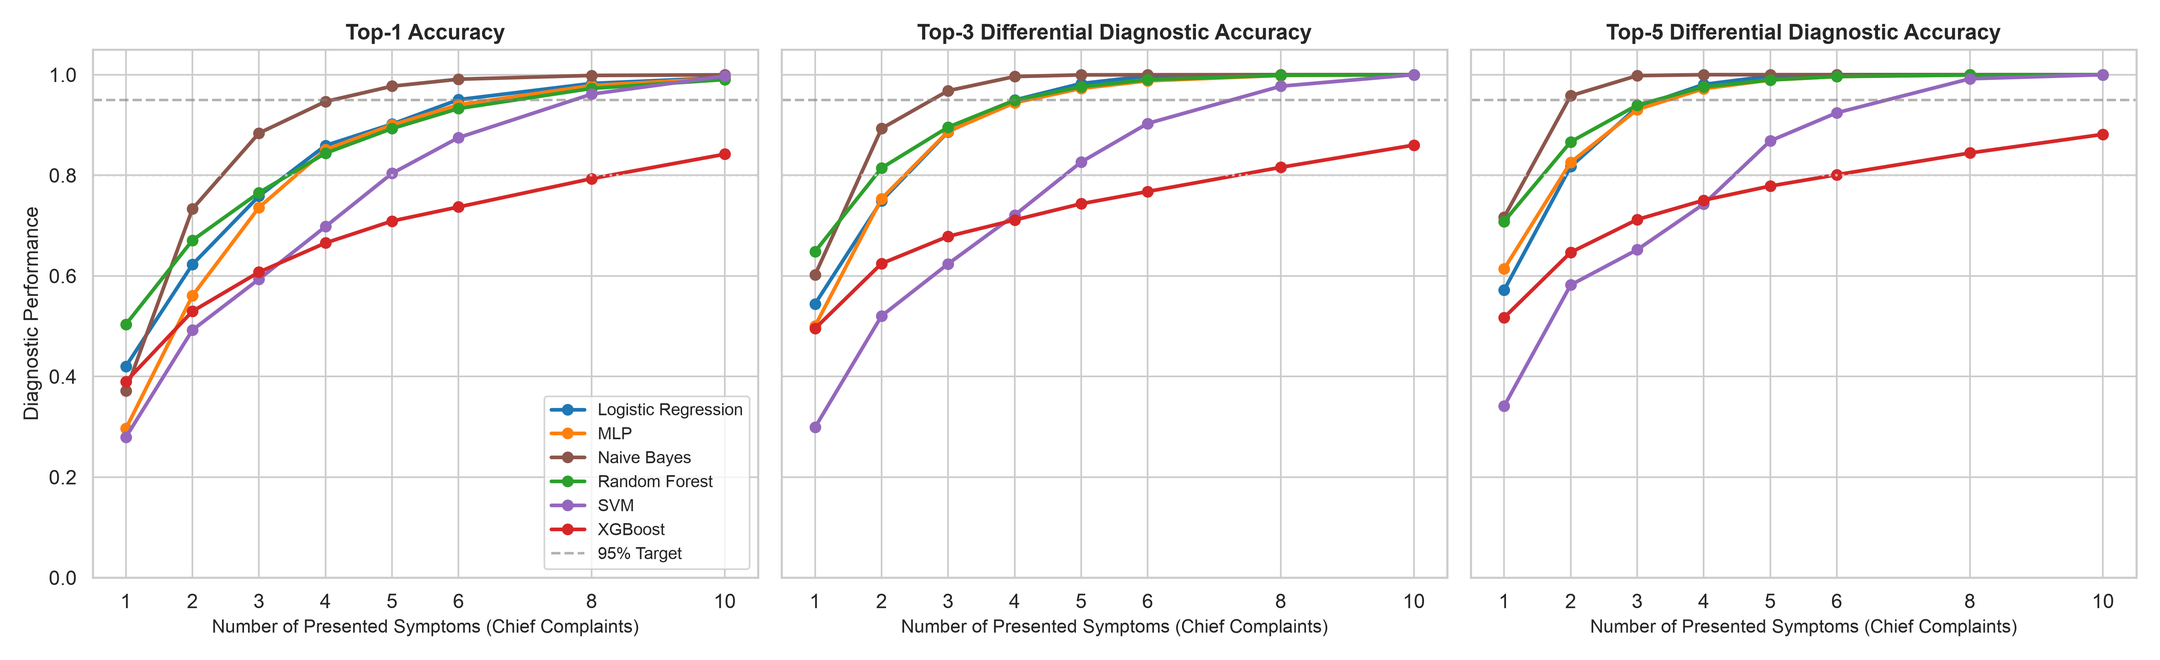
\includegraphics[width=\textwidth]{sparsity_decay_curves.png}
\caption{Diagnostic performance degradation curves under simulated patient intake sparsity ($s \in [1, 10]$ presenting chief complaints) across six model architectures evaluated under Protocol C. Left: Top-1 single-label accuracy. Centre: Top-3 differential diagnostic accuracy. Right: Top-5 differential diagnostic accuracy. The horizontal dashed line marks the 95\% operational retention threshold. \textit{Note: Curves reflect provisional Phase 5 benchmark outputs across available masking seeds; final parameter freezing awaits completed seed matrix execution.}}
\label{fig:sparsity_decay_curves}
\end{figure}

\section{Experimental Design and Stochastic Sparsity Protocol}
\label{sec:sparsity_design}
To evaluate model resilience under controlled symptom restriction on this benchmark, models were evaluated under Protocol C across restricted symptom budgets $s \in \{\text{Full}, 10, 8, 6, 5, 4, 3, 2, 1\}$ using five independent random seeds applied across all test records. For each test sample presenting $P$ positive symptoms, if $P > s$, exactly $s$ positive symptoms were selected uniformly at random while remaining symptoms were masked to zero; if $P \le s$, the sample remained unmasked. Evaluations were conducted across both the Full 132-symptom space and the Frozen 50-symptom space identified in Phase 4.

Crucially, these controlled masking experiments represent a benchmark-specific synthetic stress test designed to quantify how algorithmic architectures respond to incomplete binary feature vectors on this dataset; they do not establish clinical diagnostic efficacy in real-world patient encounters. Furthermore, the experimental outputs reported in this chapter are \textbf{provisional}, reflecting the currently available Phase 5 runs across available masking seeds. 

\begin{table}[H]
\caption{Provisional Diagnostic Resilience Under Simulated Symptom Sparsity on the Kaggle Benchmark (Protocol C, Across Available Masking Seeds)}
\label{tab:sparsity_summary}
\centering
\scriptsize
\setlength{\tabcolsep}{3pt}
\begin{tabular}{cc|cccc|cccc}
\toprule
\multirow{2}{*}{\textbf{Model}} & \multirow{2}{*}{\textbf{Budget ($s$)}} & \multicolumn{4}{c|}{\textbf{Full 132-Symptom Space}} & \multicolumn{4}{c}{\textbf{Frozen 50-Symptom Space}} \\
\cmidrule{3-10}
& & \textbf{Top-1 Acc} & \textbf{Macro-F1} & \textbf{Top-3 Acc} & \textbf{Top-5 Acc} & \textbf{Top-1 Acc} & \textbf{Macro-F1} & \textbf{Top-3 Acc} & \textbf{Top-5 Acc} \\
\midrule
\multirow{5}{*}{Log. Reg.}
& Full (7.45$\pm$3.59) & $1.000 \pm 0.000$ & $1.000 \pm 0.000$ & 1.000 & 1.000 & $0.961 \pm 0.029$ & $0.895 \pm 0.065$ & 0.987 & 0.995 \\
& 8 Symptoms  & $0.983 \pm 0.017$ & $0.960 \pm 0.035$ & 1.000 & 1.000 & $0.942 \pm 0.028$ & $0.845 \pm 0.057$ & 0.987 & 0.995 \\
& 5 Symptoms  & $0.902 \pm 0.054$ & $0.775 \pm 0.054$ & 0.983 & 0.997 & $0.755 \pm 0.066$ & $0.546 \pm 0.054$ & 0.930 & 0.976 \\
& 3 Symptoms  & $0.759 \pm 0.076$ & $0.553 \pm 0.049$ & 0.886 & 0.936 & $0.533 \pm 0.130$ & $0.284 \pm 0.063$ & 0.743 & 0.873 \\
& 1 Symptom   & $0.420 \pm 0.089$ & $0.235 \pm 0.039$ & 0.544 & 0.572 & $0.187 \pm 0.105$ & $0.070 \pm 0.028$ & 0.406 & 0.480 \\
\midrule
\multirow{5}{*}{Rand. Forest}
& Full (7.45$\pm$3.59) & $0.994 \pm 0.010$ & $0.987 \pm 0.022$ & 1.000 & 1.000 & $0.940 \pm 0.027$ & $0.844 \pm 0.057$ & 0.982 & 0.982 \\
& 8 Symptoms  & $0.973 \pm 0.018$ & $0.932 \pm 0.039$ & 0.999 & 0.999 & $0.922 \pm 0.032$ & $0.797 \pm 0.049$ & 0.975 & 0.976 \\
& 5 Symptoms  & $0.893 \pm 0.058$ & $0.771 \pm 0.070$ & 0.976 & 0.990 & $0.818 \pm 0.058$ & $0.598 \pm 0.058$ & 0.941 & 0.960 \\
& 3 Symptoms  & $0.765 \pm 0.092$ & $0.571 \pm 0.062$ & 0.896 & 0.940 & $0.584 \pm 0.116$ & $0.330 \pm 0.050$ & 0.833 & 0.912 \\
& 1 Symptom   & $0.504 \pm 0.087$ & $0.310 \pm 0.046$ & 0.648 & 0.708 & $0.240 \pm 0.127$ & $0.096 \pm 0.040$ & 0.556 & 0.629 \\
\midrule
\multirow{5}{*}{SVM (RBF)}
& Full (7.45$\pm$3.59) & $1.000 \pm 0.000$ & $1.000 \pm 0.000$ & 1.000 & 1.000 & $0.939 \pm 0.031$ & $0.844 \pm 0.069$ & 0.963 & 0.970 \\
& 8 Symptoms  & $0.961 \pm 0.029$ & $0.904 \pm 0.051$ & 0.977 & 0.992 & $0.920 \pm 0.038$ & $0.803 \pm 0.068$ & 0.956 & 0.968 \\
& 5 Symptoms  & $0.804 \pm 0.087$ & $0.618 \pm 0.045$ & 0.826 & 0.868 & $0.769 \pm 0.054$ & $0.517 \pm 0.054$ & 0.809 & 0.873 \\
& 3 Symptoms  & $0.593 \pm 0.112$ & $0.374 \pm 0.056$ & 0.624 & 0.652 & $0.523 \pm 0.132$ & $0.260 \pm 0.055$ & 0.548 & 0.601 \\
& 1 Symptom   & $0.279 \pm 0.123$ & $0.150 \pm 0.046$ & 0.299 & 0.341 & $0.206 \pm 0.125$ & $0.079 \pm 0.032$ & 0.253 & 0.331 \\
\midrule
\multirow{5}{*}{MLP}
& Full (7.45$\pm$3.59) & $1.000 \pm 0.000$ & $1.000 \pm 0.000$ & 1.000 & 1.000 & $0.977 \pm 0.024$ & $0.934 \pm 0.057$ & 0.990 & 1.000 \\
& 8 Symptoms  & $0.978 \pm 0.018$ & $0.952 \pm 0.040$ & 0.999 & 1.000 & $0.957 \pm 0.029$ & $0.883 \pm 0.054$ & 0.990 & 1.000 \\
& 5 Symptoms  & $0.900 \pm 0.049$ & $0.792 \pm 0.066$ & 0.973 & 0.989 & $0.836 \pm 0.053$ & $0.647 \pm 0.040$ & 0.948 & 0.986 \\
& 3 Symptoms  & $0.736 \pm 0.106$ & $0.580 \pm 0.065$ & 0.887 & 0.931 & $0.618 \pm 0.086$ & $0.385 \pm 0.041$ & 0.811 & 0.893 \\
& 1 Symptom   & $0.296 \pm 0.119$ & $0.215 \pm 0.041$ & 0.500 & 0.614 & $0.206 \pm 0.107$ & $0.090 \pm 0.033$ & 0.439 & 0.519 \\
\midrule
\multirow{5}{*}{XGBoost}
& Full (7.45$\pm$3.59) & $0.884 \pm 0.045$ & $0.680 \pm 0.109$ & 0.903 & 0.920 & $0.854 \pm 0.037$ & $0.580 \pm 0.078$ & 0.909 & 0.924 \\
& 8 Symptoms  & $0.793 \pm 0.045$ & $0.547 \pm 0.086$ & 0.816 & 0.844 & $0.777 \pm 0.045$ & $0.471 \pm 0.067$ & 0.844 & 0.875 \\
& 5 Symptoms  & $0.709 \pm 0.055$ & $0.435 \pm 0.065$ & 0.743 & 0.779 & $0.634 \pm 0.103$ & $0.326 \pm 0.072$ & 0.722 & 0.774 \\
& 3 Symptoms  & $0.607 \pm 0.063$ & $0.339 \pm 0.055$ & 0.679 & 0.712 & $0.509 \pm 0.116$ & $0.229 \pm 0.066$ & 0.621 & 0.676 \\
& 1 Symptom   & $0.390 \pm 0.077$ & $0.209 \pm 0.040$ & 0.495 & 0.517 & $0.217 \pm 0.111$ & $0.091 \pm 0.031$ & 0.373 & 0.487 \\
\midrule
\multirow{5}{*}{Naive Bayes}
& Full (7.45$\pm$3.59) & $1.000 \pm 0.000$ & $1.000 \pm 0.000$ & 1.000 & 1.000 & $0.864 \pm 0.094$ & $0.883 \pm 0.082$ & 0.965 & 0.972 \\
& 8 Symptoms  & $0.999 \pm 0.004$ & $0.998 \pm 0.004$ & 1.000 & 1.000 & $0.859 \pm 0.085$ & $0.877 \pm 0.075$ & 0.965 & 0.972 \\
& 5 Symptoms  & $0.977 \pm 0.022$ & $0.969 \pm 0.023$ & 1.000 & 1.000 & $0.832 \pm 0.084$ & $0.834 \pm 0.073$ & 0.964 & 0.972 \\
& 3 Symptoms  & $0.884 \pm 0.053$ & $0.829 \pm 0.043$ & 0.968 & 0.998 & $0.722 \pm 0.077$ & $0.667 \pm 0.060$ & 0.926 & 0.970 \\
& 1 Symptom   & $0.372 \pm 0.081$ & $0.313 \pm 0.033$ & 0.602 & 0.717 & $0.145 \pm 0.047$ & $0.137 \pm 0.020$ & 0.489 & 0.658 \\
\bottomrule
\end{tabular}
\begin{flushleft}
\scriptsize
\textit{Note: Results report mean $\pm$ standard deviation across evaluated masking seeds. These values are provisional pending complete model-by-budget-by-seed matrix completion. Baseline full-input OOF Macro-F1 scores exhibit variations across specific cross-validation splits and model configurations (e.g., Random Forest: 0.9866--0.9963; MLP: 0.9803--1.0000; SVM: 0.9915--1.0000; XGBoost: 0.6802--0.9137). Neither Table~\ref{tab:sparsity_summary} nor Figure~\ref{fig:sparsity_decay_curves} should be regarded as frozen parameters prior to final experimental reconciliation.}
\end{flushleft}
\end{table}

\section{The Differential Diagnostic Safeguard Under Sparsity}
\label{sec:differential_safeguard}
As documented in Table~\ref{tab:sparsity_summary} and \cref{fig:sparsity_decay_curves}, progressive symptom restriction induces two contrasting empirical regimes across the evaluated models:
\begin{enumerate}
    \item \textbf{Single-Label Accuracy Collapse}: Top-1 accuracy experiences a steep decline as presenting symptoms fall below $s = 5$. At $s = 3$ presenting symptoms (simulating acute reporting restriction), Top-1 accuracy declines to 75.9\% (Macro-F1: 55.3\%) for Logistic Regression, 76.5\% (Macro-F1: 57.1\%) for Random Forest, and 73.6\% (Macro-F1: 58.0\%) for MLP on the Full 132 space. At $s = 1$, Top-1 accuracy falls into the 27.9\%--50.4\% range (Macro-F1: 15.0\%--31.3\%) across all models.
    \item \textbf{Differential Diagnostic Buffer}: In sharp contrast, multi-candidate ranking demonstrates remarkable resilience. At $s = 3$ symptoms, \textbf{Top-3 diagnostic accuracy remains above 88.6\%} for Logistic Regression (88.6\%), Random Forest (89.6\%), and MLP (88.7\%), with Naive Bayes reaching 96.8\%, while \textbf{Top-5 accuracy exceeds 93.0\%} across these architectures. Even at $s = 2$ presenting symptoms, Top-5 inclusion remains between 81.7\% and 86.7\% for the leading models.
\end{enumerate}

These empirical observations highlight the vital safeguard provided by differential candidate ranking over rigid single-label classification under simulated sparsity: presenting an ordered candidate list (Top-3 to Top-5) ensures that the true disease label is captured in over 93\% of evaluated cases under moderate symptom restriction on this benchmark, providing a candidate buffer prior to confirmatory diagnostics.

\section{Architectural Sensitivity and Representation Resilience}
\label{sec:arch_sensitivity}
\begin{itemize}
    \item \textbf{Additive vs.\ Partitioning Models}: Linear (Logistic Regression) and neural (MLP) architectures degrade gracefully under moderate sparsity ($s \ge 4$), as their additive decision boundaries aggregate evidence from whatever subset of features is present. Tree ensembles (Random Forest, XGBoost) experience steeper drops when higher-level tree split nodes interrogate features that the patient omitted, though Random Forest maintains higher Top-1 retention at extreme sparsity ($s=1$, 50.4\%) due to bootstrap feature subsampling.
    \item \textbf{Kernel and Probabilistic Baselines}: SVM (RBF) degrades sharply at $s \le 3$ (Top-1 59.3\% at $s=3$ and 27.9\% at $s=1$) because geometric distances in the 132-dimensional kernel space are distorted by large fractions of zeroed dimensions. Conversely, Naive Bayes retains exceptionally high Top-3 and Top-5 candidate retention under moderate sparsity ($s=5$, Top-3 100.0\%), though its single-label accuracy collapses at $s=1$ (37.2\%).
    \item \textbf{Representation Generalization (132 vs.\ 50 Features)}: Evaluating models trained on the Frozen 50-symptom space revealed that retaining only core consensus features achieves comparable sparsity decay trajectories to the uncompressed 132-symptom model down to $s=5$. Below $s=4$, the reduced feature pool accelerates degradation because masking active symptoms leaves fewer alternative informative features within the 50-symptom subspace.
\end{itemize}

In summary, the degradation profiles underscore that candidate differential ranking mitigates information loss when symptom reporting is incomplete. However, final confirmation of these trajectories requires the ongoing full seed-by-budget re-run and ultimate validation against real-world clinical patient registries.
